\begin{figure}[htbp]
\centering
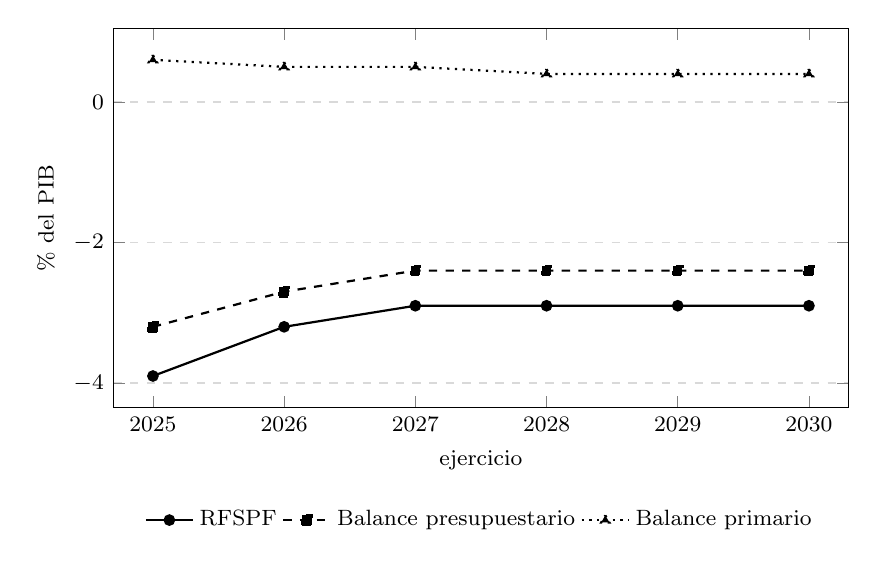
\begin{tikzpicture}
\begin{axis}[
  width=0.9\textwidth, height=6.4cm,
  xlabel={ejercicio}, ylabel={\% del PIB},
  legend style={font=\footnotesize, at={(0.5,-0.24)}, anchor=north,
                 legend columns=-1, draw=none},
  tick label style={font=\footnotesize},
  label style={font=\footnotesize},
  x tick label style={/pgf/number format/1000 sep={}},
  ymajorgrids=true, grid style={dashed, gray!30},
  enlarge x limits=0.06,
  cycle list={{solid,mark=*}, {dashed,mark=square*}, {dotted,mark=triangle*}, {dashdotted,mark=diamond*}},
  xtick=data,
]
\addplot+[thick, mark size=1.7pt] coordinates {(2025,-3.9) (2026,-3.2) (2027,-2.9) (2028,-2.9) (2029,-2.9) (2030,-2.9)};
\addlegendentry{RFSPF}
\addplot+[thick, mark size=1.7pt] coordinates {(2025,-3.2) (2026,-2.7) (2027,-2.4) (2028,-2.4) (2029,-2.4) (2030,-2.4)};
\addlegendentry{Balance presupuestario}
\addplot+[thick, mark size=1.7pt] coordinates {(2025,0.6) (2026,0.5) (2027,0.5) (2028,0.4) (2029,0.4) (2030,0.4)};
\addlegendentry{Balance primario}
\end{axis}
\end{tikzpicture}
\caption{Los flujos fiscales en el escenario oficial, 2025--2030}
\label{fig:F12_1}
\par\vspace{2pt}\footnotesize Fuente: elaboración propia del ITED con información de la SHCP, CGPE 2025, Anexo III.2, p. 85. El acervo se mantiene plano en 51.4 \% del PIB los seis años (cuadro 12.2); el ajuste ocurre en el flujo. El CGPE 2025 se publicó sin capa de texto; las cifras se leyeron de la página renderizada y se validaron por identidad contable.
\end{figure}
